\documentclass[letter, 12pt]{article}

\usepackage{amsmath,amsthm,amssymb}
\usepackage{fancyhdr}
\usepackage{geometry}
\usepackage{enumerate}
\usepackage{enumitem}
\usepackage{listings}
\usepackage{algorithm}
\usepackage{hyperref}
\usepackage{algorithmic}
\usepackage{eqparbox}
\usepackage{float}
\usepackage{bm}
\usepackage{bbm}
\usepackage{mathtools}

\author{Shengjie Li}
\title{Homework 3}

\pagestyle{fancy}
\fancyhf{} 
\lhead{Shengjie Li \\ RUID: 188008047}
\cfoot{\thepage} 
\renewcommand{\headrulewidth}{1pt}
\renewcommand{\headwidth}{\textwidth}
\renewcommand\algorithmiccomment[1]{%
	\hfill\#\ \eqparbox{COMMENT}{#1}%
}
\newlist{subquestion}{enumerate}{1}
\setlist[subquestion, 1]{label = \alph*)}
\DeclareMathOperator*{\argmax}{arg\,max}
\DeclareMathOperator*{\argmin}{arg\,min}

\setlength\parindent{0pt}

% margin adjustment
\addtolength{\textwidth}{1in}
\addtolength{\oddsidemargin}{-0.5in}
\addtolength{\evensidemargin}{-0.5in}
\addtolength{\topmargin}{-.5in}
\addtolength{\textheight}{1.0in}
\setlength\parindent{0cm}

\begin{document}
	\centerline{Homework 3}
	\begin{enumerate}[wide = 0pt, label = \textbf{Problem \arabic*:}]
		\item {\ } 
		\begin{subquestion}
			\item {\textbf{Solution:} }
			\par{The histogram of the 1000 generated random variables is shown in Fig \ref{fig:histo}.}
			\begin{figure}[H]
				\centering
				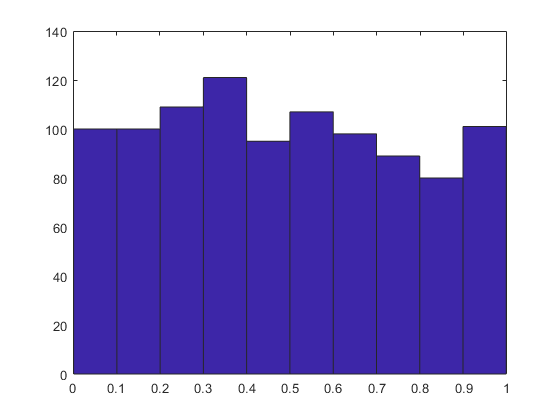
\includegraphics[width=0.7\textwidth]{figs/histogram.png}
				\caption{Histogram of 1000 random variables}
				\label{fig:histo}
			\end{figure}
			\par{According to the Law of Large Numbers, $ \mathbb{E}[K_h(X-x)] \approx \frac{K_h(X - x_1) + K_h(X - x_2) + \dots + K_h(X - x_n)}{n} \approx f(x) $.}
			\par{When we approximate the pdf using the Gaussian kernel, \[ K_h(X) = \frac{e^{-\frac{1}{2h}x^2}}{\sqrt{2 \pi h}}. \] }
			\par{The results are shown in Fig \ref{fig:pdf-gaussian}.}
			\par{We can see from Fig \ref{fig:pdf-gaussian} that when the $ h $ is large, the model underfit the pdf, which is not close enough. As the $ h $ is decreasing, the support of the random variable becomes closer to $ [0, 1] $, and the approximation of pdf becomes more zigzag around 1, starts to overfit.}
			\begin{figure}[H]
				\centering
				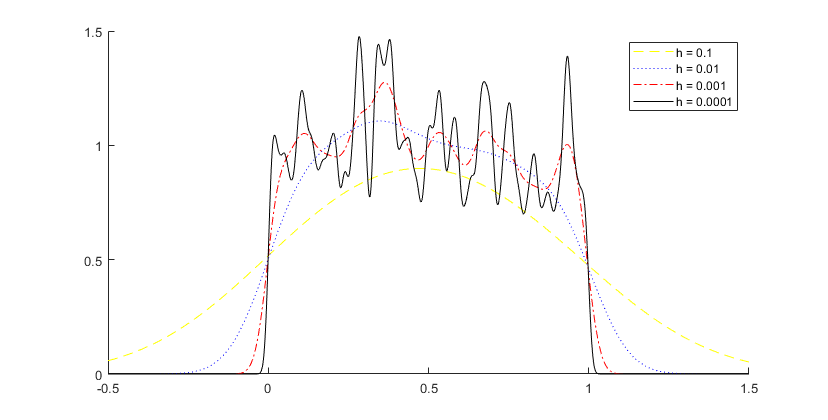
\includegraphics[width=\textwidth]{figs/pdf-gaussian.png}
				\caption{Approximation using Gaussian kernel under different $ h $s.}
				\label{fig:pdf-gaussian}
			\end{figure}
		
			\item {\textbf{Solution:} }
			\par{When we approximate the pdf using the Laplacian kernel, \[ K_h(X) = \frac{e^{-\frac{1}{2h}x^2}}{\sqrt{2 \pi h}}. \] }
			\par{The results are shown in Fig \ref{fig:pdf-laplacian}.}
			\begin{figure}[H]
				\centering
				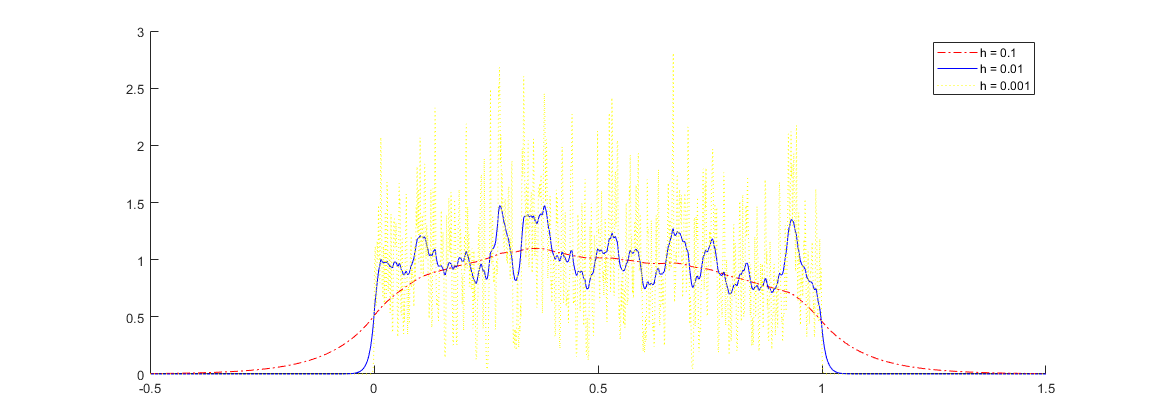
\includegraphics[width=\textwidth]{figs/pdf-laplacian.png}
				\caption{Approximation using Laplacian kernel under different $ h $s.}
				\label{fig:pdf-laplacian}
			\end{figure}
		\end{subquestion}
		
		\item{\ }
		\begin{subquestion}
			\item {\textbf{Solution:} }
			\par{By solving this minimization problem:  \[\min_{\phi}\{\sum_{X_i \in \texttt{stars}}(1 - \phi(X_i))^2 + \sum_{X_j \in \texttt{circles}}(1 + \phi(X_j))^2 + \lambda || \phi(X) ||^2\}, \] the idea is to try to minimize the loss.}
			\par{Define $ V $, the space of functions that generated by the Gaussian kernel
				\[ K(X, Y) = e^{-\frac{1}{h}||X-Y||^2} = e^{-\frac{1}{h}\{(x_1-y_1)^2+(x_2-y_2)^2\}} .\]}
			\par{Define $ \phi(X):z \rightarrow K(x, z) $, $ z \in \mathbb{R}^2 $, $ K(x, z) \in V $.}
			\par{In the vector space, $ g(x) = \sum_{i = 1}^{m} \alpha _i K(x, z_i) $, $ h(x) = \sum_{i = 1}^{m'} \beta _i K(x, {z'}_i) $.}
			\par{Define the inner product:}
			\[ <g(x), h(x)> = \sum_{i = 1}^{m}\sum_{j = 1}^{m'} \alpha _i \beta _j K(z_i, {z'}_j) .\]
			\par{Then we are trying to solving \[\min_{g(x) \in V}\{\sum_{X_i \in \texttt{stars}}(1 - g(X_i))^2 + \sum_{X_j \in \texttt{circles}}(-1 - g(X_j))^2 + \lambda || g(X) ||^2\}, \text{where $ g(X) = <g(X), g(X)> $}.\]}
			\par{According to the theorem, the best choice would be $ m = N, z_i = x_i $.}
			\par{Thus, $ g(x) = \sum_{i = 1}^{m} \alpha _i K(x, x_i) + \sum_{i = 1}^{m'} \beta _i K(x, {x'}_i) $, where $ x_i $s are data of stars, $ x_i' $s are data of circles.}
			\par{If we concatenate the input data, the inner product would be:
			\[ <g(x), g(x)> = \sum_{i = 1}^{m}\sum_{j = 1}^{m'} \alpha _i \alpha _j K(x_i, {x'}_j) = \alpha ^T K \alpha,\]}
			\par{and $ g(x) $ would be: $ g(x) = K \alpha .$ $ K $ is positive definite and symmetric.}
			\par{Denote the original class of the input data by $ b $, then the minimization we are trying to solve becomes: 
			\[ min(||b - K \alpha||^2 + \lambda \alpha ^T K \alpha) .\]}
			\par{We let the partial derivative equal to 0, we get $ \alpha = (\lambda I + K)^{-1}b .$}
			\par{We hereby successfully turned the question. }
			\item {\textbf{Solution:} }
			\par{Now we can just put the new point $ X_{new} $ into $ g(x) = \alpha_1 K(x, x_i) + \dots + \alpha_m K(x, x_m) + \alpha_1 K(x, {x'}_i) + \dots + \alpha_{m'} K(x, {x'}_{m'}) $. }
			\par{If $ g(X_{new}) > 0 $, we call it a star. Otherwise we call it a circle.}
			\item {\textbf{Solution:} }
			\par{The boundary for the two classes would be lying on where $ g(x) = 0 $. The results are shown in Fig \ref{fig:fig-gaussian-10} and Fig \ref{fig:fig-gaussian-lambda}.}
			\item {\textbf{Solution:} }
			\begin{figure}[H]
				\centering
				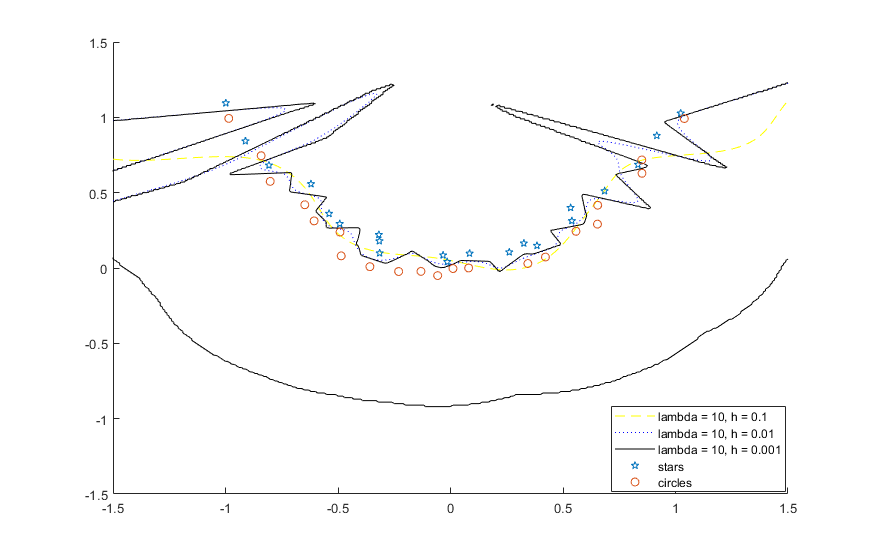
\includegraphics[width=\textwidth]{figs/fig-gaussian-10.png}
				\caption{The boundary under different values of $ h $.}
				\label{fig:fig-gaussian-10}
			\end{figure}
			\begin{figure}[H]
				\centering
				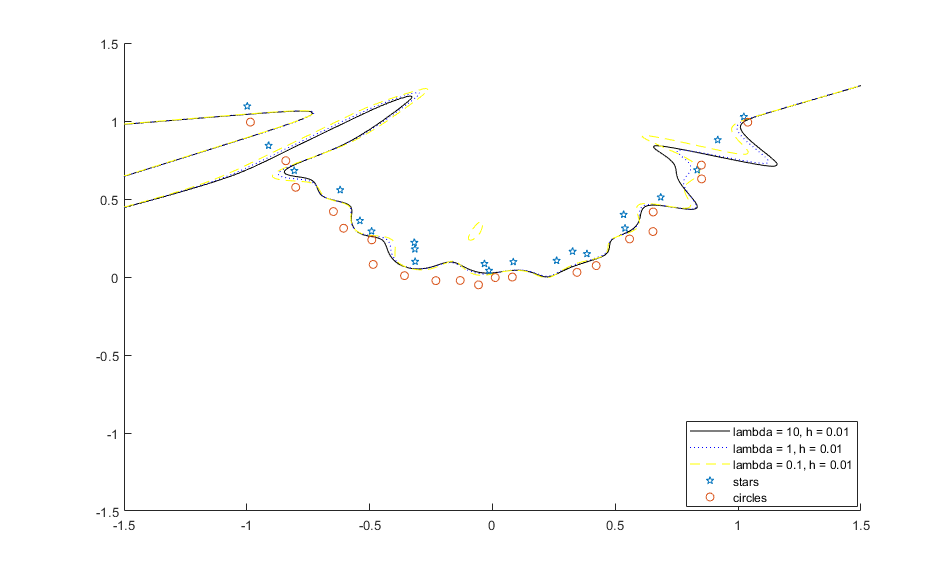
\includegraphics[width=\textwidth]{figs/fig-gaussian-lambda.png}
				\caption{The boundary under different values of $ \lambda $.}
				\label{fig:fig-gaussian-lambda}
			\end{figure}
			\item {\textbf{Solution:} }
			\par{When using the simpler kernel function \[K(X, Y) = (1 + x_1 y_1 + x_2 y_2)^2 ,\] we can still use the theorem.}
			\par{We can actually use the same $ g(x) $, so that if given a new point $ X_{new} $, if $ g(X_{new}) > 0 $, we call it a star. Otherwise we call it a circle.}
			\par{The results for different values of $ \lambda $ are shown in Fig \ref{fig:simpler-kernel}.}
			\par{Some examples of functions $ \phi(X) $ are:}
			\begin{itemize}
				\item {\[g(x) = C_0 + x_1 y_1 + x_2 y_2 + \dots + x^2 y^2 \]}
				\item {\[g(x) = C_0 + C_1 x_1 + C_1 x_2 + C_2 x_1 x_2 + d_1 x_1^2 + d_2 x_2^2\]}
			\end{itemize}
			\begin{figure}[H]
				\centering
				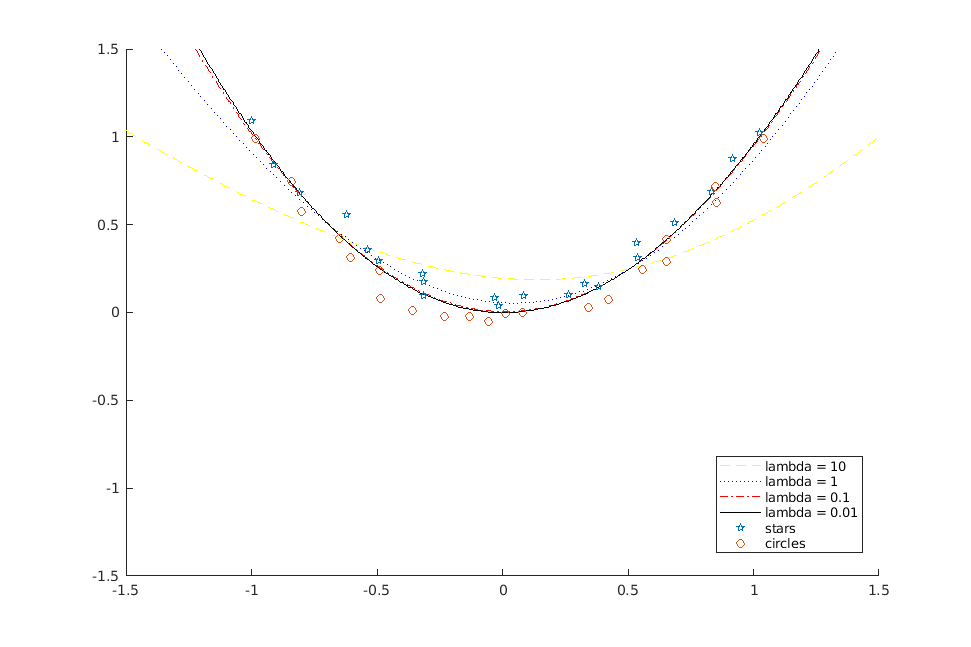
\includegraphics[width=\textwidth]{figs/simple-kernel.png}
				\caption{The boundary under different values of $ \lambda $.}
				\label{fig:simpler-kernel}
			\end{figure}
		\end{subquestion}
	\end{enumerate}
\end{document}
